\documentclass[a4paper]{scrartcl}

%% Language and font encodings
\usepackage[english]{babel}
\usepackage[utf8x]{inputenc}
\usepackage[T1]{fontenc}

%% Sets page size and margins
\usepackage[a4paper,top=2cm,bottom=3cm,left=3cm,right=2cm,marginparwidth=1.75cm]{geometry}

%% Useful packages
\usepackage{amsmath}
\usepackage{graphicx}
\usepackage{subcaption}
\usepackage[colorinlistoftodos]{todonotes}
\usepackage[colorlinks=true, allcolors=blue]{hyperref}
\usepackage{placeins}
\usepackage{siunitx}
\usepackage{sidecap}
\usepackage{float}
\usepackage[format=plain]{caption}
\DeclareSIUnit\atmosphere{atm}

\title{Computational Motor Control - Lab 4}
\author{Florian Kaufmann \and Octave Martin \and Matthias Tsai}

\begin{document}
\maketitle

\section{Modelling the lamprey CPG with phase oscillators}
\subsection{Parameter values for the model (6a.)}

We studied how lamprey CPGs could be modeled with a chain of phase oscillators and first started to explore this model by implementing and simulating different kinds chains of phase oscillators with various parameters. The parameters varied were the number of oscillators, the gradient of frequencies between them and the coupling strength between oscillators. To start off, we chose 10 oscillators, a frequency gradient of $\pi /6$ and a coupling strength of 7 to get an example of a phase-locked chain of oscillators (see Figure \ref{fig:f6a-standard}). From the plots, one can observe that the phase differences between the oscillators all stabilize to constant values and the oscillators visibly synchronize (left plot) by all adopting the same frequency despite of the intrinsic frequency gradient(right plot).

\begin{figure}[!b]
	\centering
	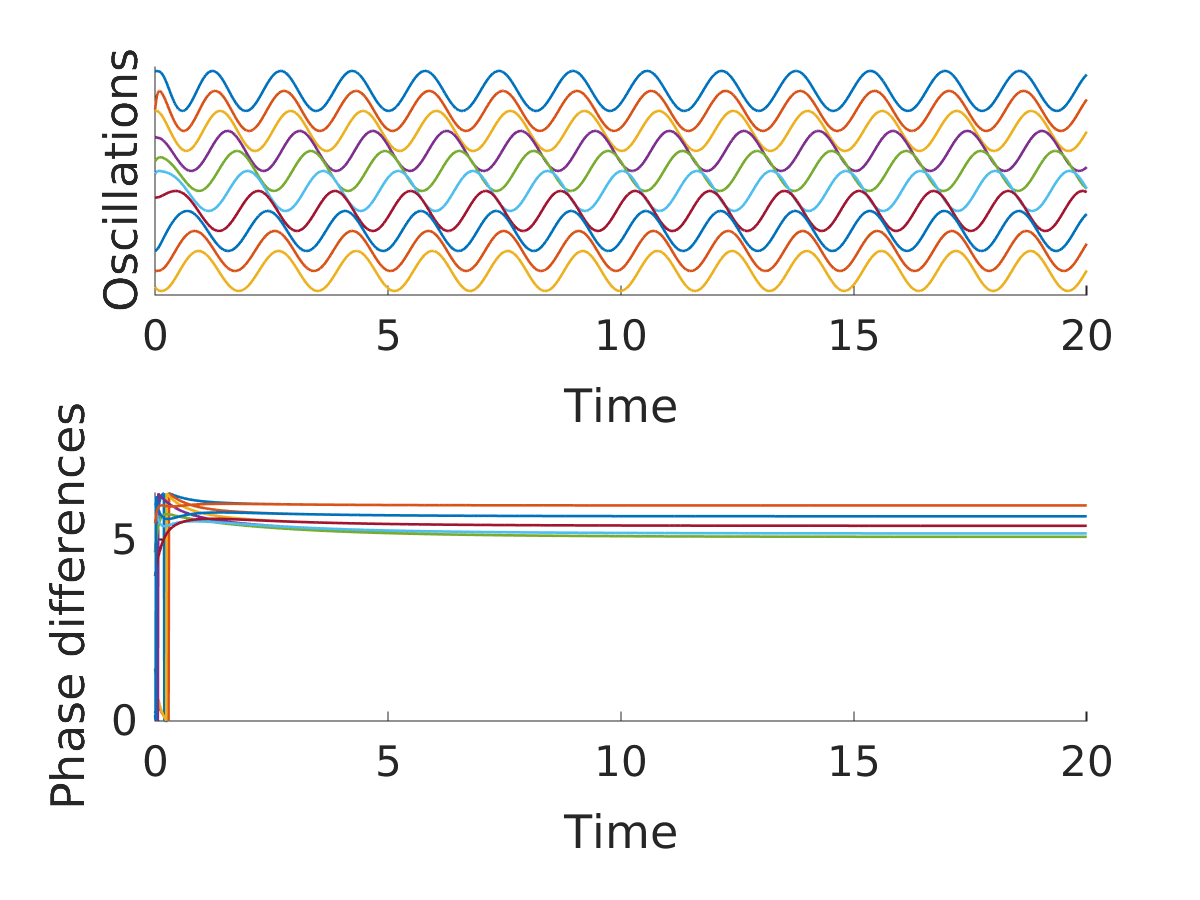
\includegraphics[width=0.5\textwidth]{fig/chain_phase_oscil-6a_stable.png}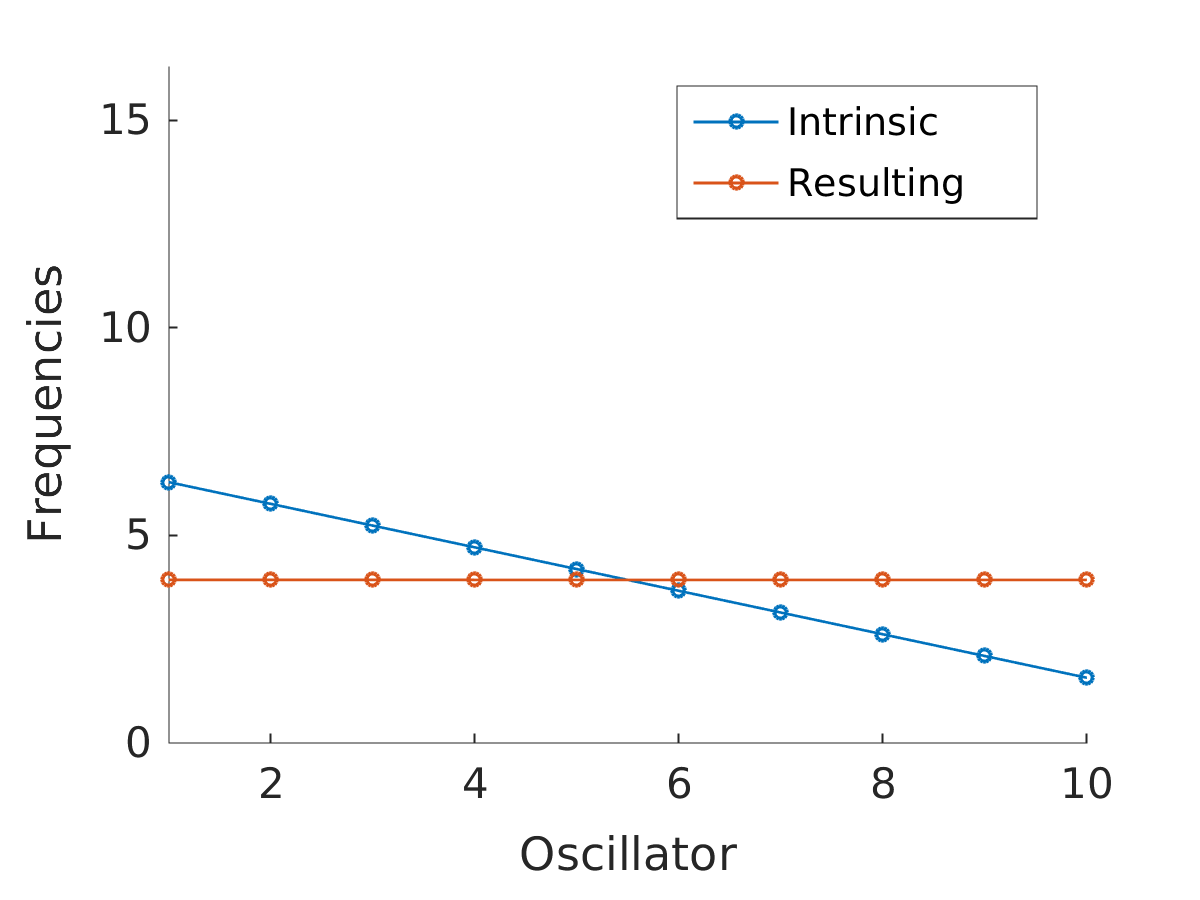
\includegraphics[width=0.5\textwidth]{fig/chain_phase_oscil_freq-6a_stable.png}
	\caption{Simulation of a chain of 10 phase oscillators with frequency gradient of $\pi /6$ and coupling strength of 7. Left: Simulated oscillations and phase differences of the oscillators over time.  Right: Plot of intrinsic frequencies and resulting frequencies from the simulation.}
	\label{fig:f6a-standard}
\end{figure}

Next, we used our analytical formula to sufficiently modify the value of one parameter at a time in order to lose the phase-locked behaviour of the chain of oscillators. First, the coupling strength was modified and reduced to 4 (see Figure \ref{fig:f6a-unstablecoupling}), and as predicted by our analytical model, the phase locking was lost. Interestingly, the chain of oscillators seems to have converged on two distinct frequencies, with the upper half of the chain synchronizing on a higher frequency as the lower part of the chain, with the central oscillators (especially the green one) experiencing an increased instability by being localized at the interface between these two subsystems.

\begin{figure}[!t]
	\centering
	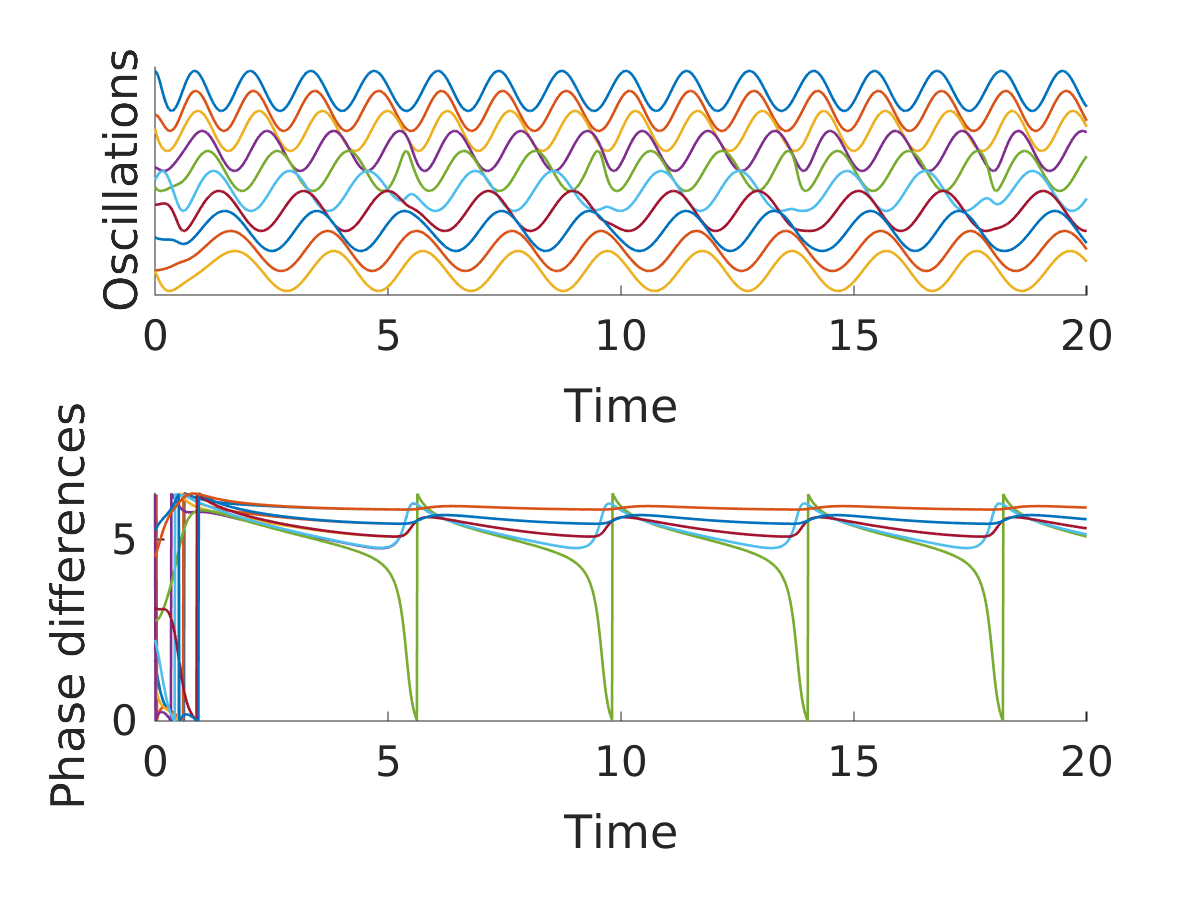
\includegraphics[width=0.5\textwidth]{fig/chain_phase_oscil-6a_unstable.png}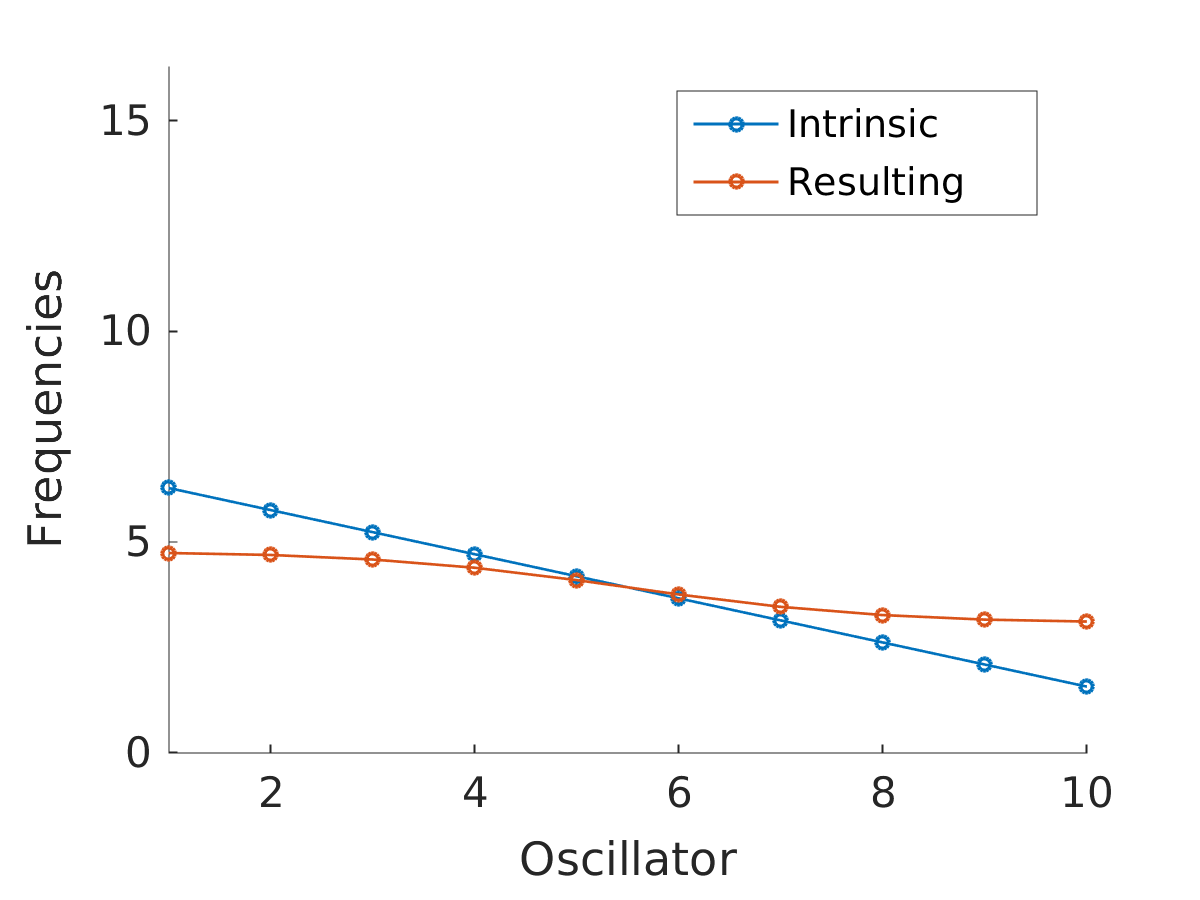
\includegraphics[width=0.5\textwidth]{fig/chain_phase_oscil_freq-6a_unstable.png}
	\caption{Simulation of a chain of 10 phase oscillators with frequency gradient of $\pi /6$ and coupling strength of 4. Left: Simulated oscillations and phase differences of the oscillators over time. Right: Plot of intrinsic frequencies and resulting frequencies from the simulation.}
	\label{fig:f6a-unstablecoupling}
\end{figure}

Similar loss of phase locking was also observed, if our initial phase locked oscillator chain was modified to either raise the frequency gradient to $\pi /5$ or to raise the number of oscillators to 11. This isn't very surprising, because by looking at the phase locking inequality condition using the parameters of our synchronized oscillator chain, one can predict that already a small change of one parameter in the wrong direction would change the sign of the inequality. This is because our chosen standard parameters are already very close to the threshold at which the system loses its phase locking dynamic.

\begin{equation}
	coupling \_ strength = 7 > 6.545 =\frac{\pi \cdot 10^{2}}{6 \cdot 8} = \frac{frequency \_ gradient \cdot Noscils^2}{8}
\end{equation}

In order to get a better idea about how the parameters influence the phase locking, we compared if and how phase differences between oscillators stabilized during the simulations. The standard deviation measures the spread of the variables, therefore the standard deviation of the phase differences between oscillators is constant, if they are synchronized. The standard deviation of the phase differences between oscillators was therefore plotted throughout the simulations using different values for the investigated parameters (see Figure \ref{fig:f6a-phaseSTD}). The first four figures represent such standard deviations of the phase differences between oscillators as a function of time for different values of the system parameters. The simulations were performed for models with linear frequency gradients along the spinal cord and for identical initial conditions. The left column corresponds to models with 10 oscillators and the central column corresponds to models with 20 oscillators. Along the upper row the coupling strength was varied between 1 and 5. Along the lower row the intrinsic frequency gradient was varied between -0.2\,rad/step to -0.001\,rad/step. 

The fifth figure shows Arnold tongues representing the necessary values for coupling strength and frequency gradient for phase locking. The phase locking is verified for couples in the region above the straight lines. The limit condition for a model with 10 oscillators is represented with a dashed line and the limit condition for a model with 20 oscillators is represented with a plain line. Each couple of parameters tested is also plotted, with circles for the variation of the coupling strength (first row) and stars for the variation of the frequency drift (second row).

As expected the simulations and the analytical predictions depicted by the Arnold tongues for phase locking are coherent. For the models with 10 oscillators the simulation for three of the parameter couples present phase locking while only two are phase-locked for the 20 oscillator models. The parameter couple that is phase-locked for 10 oscillators but not for 20 has a coupling strength of 2 and a frequency gradient of -0.2\,rad/step. It is plotted in orange in the four left plots and corresponds to the point in the center of the five points plotted in the Arnold tongue figure.


\begin{figure}[!t]
	\hspace{0.4 cm}\textbf{Chains of 10 oscillators}\hspace{0.9 cm}\textbf{Chains of 20 oscillators}
	
	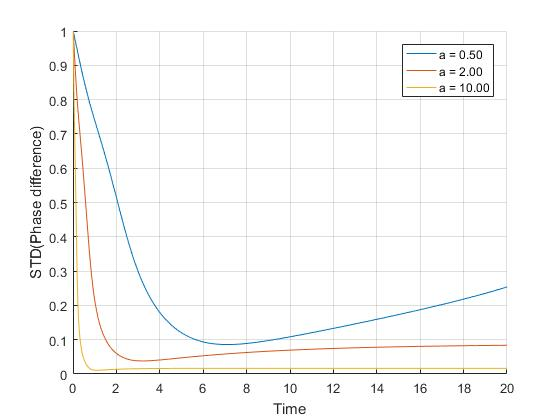
\includegraphics[width=0.33\textwidth]{results/6.a/N10_E_const.jpg}
	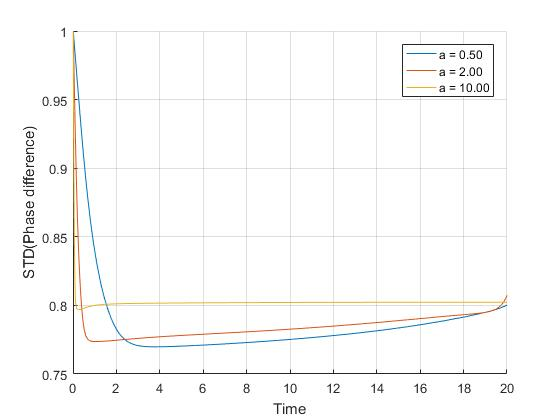
\includegraphics[width=0.33\textwidth]{results/6.a/N20_E_const.jpg}
	
	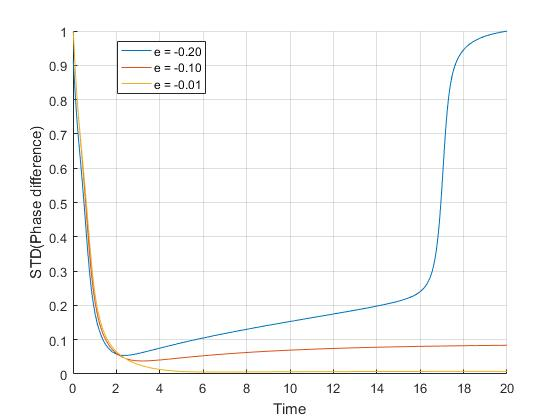
\includegraphics[width=0.33\textwidth]{results/6.a/N10_A_const.jpg}
	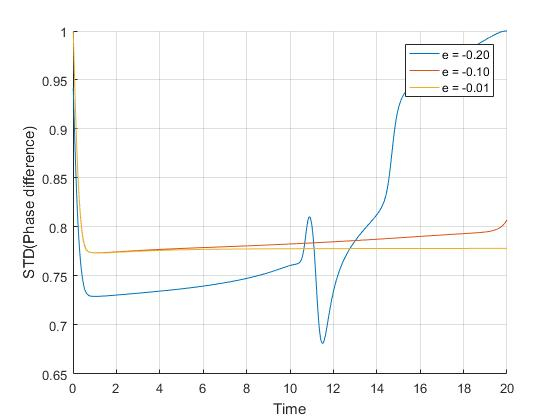
\includegraphics[width=0.33\textwidth]{results/6.a/N20_A_const.jpg}
	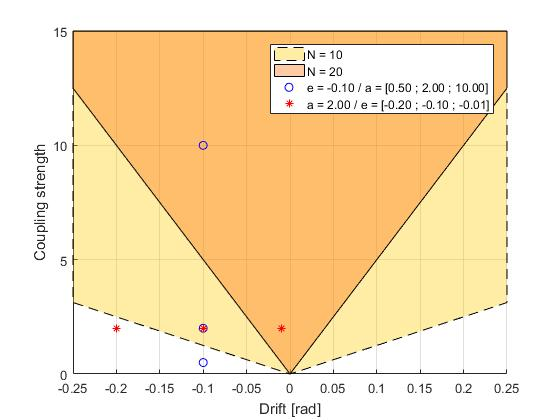
\includegraphics[width=0.33\textwidth]{results/6.a/ArnoldTongue.jpg}
	\caption{Comparison of the standard deviations of the phase gradients between oscillators throughout 20 seconds simulations with different values for the parameters of the CPG model. The two left plots use simulations using chains of 10 oscillators and the two central plots use simulations using chains of 20 oscillators. The upper left and upper central plots use simulations with different values for the coupling strength between oscillators. The lower left and lower central plots use simulations with different values for the linear intrinsic frequency gradient between oscillators. The plot on the right depicts the Arnold tongues corresponding to the parameter subspaces for which phase locking is achieved for chains of either 10 or 20 oscillators. The parameters defining the Arnold tongues are the intrinsic frequency gradients and the coupling strengths between oscillators. Some points are also depicted in the Arnold tongue figure that correspond to the parameter values that were simulated in the four other plots.}
	\label{fig:f6a-phaseSTD}
\end{figure}


\subsection{Non-linear intrinsic frequency gradient (6.b)}

Previous simulations have shown that a linear intrinsic frequency gradient leads to a quadratic phase difference between adjacent oscillators once a stable state has been reached and a sigmoid-like phase difference with respect to the first oscillator of the chain (see Figure \ref{prop}). The stable phase difference with oscillator 1 was found using the cumulative sum of the phase differences between adjacent oscillators. The phase difference between the first and last oscillators is approximatively $2\pi$ i.e. they are in phase as sinus function is $2\pi$-periodic. This correspond to a travelling wave with wavelength equal to the length of the lamprey spinal cord.

In order to study how a different type of intrinsic frequency distribution would influence the model, a simulation was run using a polynomial function to define the intrinsic frequencies of the oscillators (see Figure \ref{stand}). This lead to a sinusoid-like stable phase difference between adjacent oscillators. The stable phase difference with oscillator 1 was found using the cumulative sum of the phase differences between adjacent oscillators. Including the first and last oscillator there are 5 locations where the phase difference with oscillator 1 is null. These points are in phase with each other. This correspond to a standing wave along the lamprey with 5 nodes and therefore 4 anti-nodes.

This is an interesting result, but it is known from biology that the lamprey has constant phase difference between adjacent oscillators while swimming, leading to a linear phase difference to the first oscillator. The linear intrinsic frequency gradient produces a non constant stable phase difference between  adjacent oscillators, which can be seen in figures \ref{3d} and \ref{3e}. It was therefore attempted to reproduce that behaviour with a custom intrinsic frequency distribution (see Figure \ref{3a}). This linear gradient produced a constant phase difference between adjacent oscillators and a linear phase difference with respect to the first oscillator (see Figure \ref{3b}). The simulation that stabilized to a straight wavefront is shown in figure \ref{3e}.

\vspace{1cm}

\begin{figure}[h]
	\centering
	\begin{subfigure}[b]{0.49\textwidth}
		\centering
		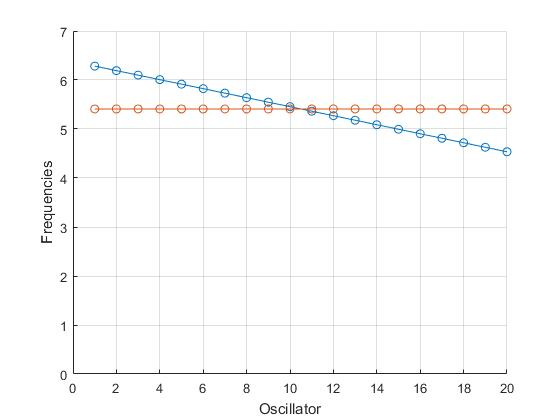
\includegraphics[width=\textwidth]{results/6.b/propaWaveFreq.jpg}
		\caption{}
	\end{subfigure}
	\centering
	\begin{subfigure}[b]{0.49\textwidth}
		\centering
		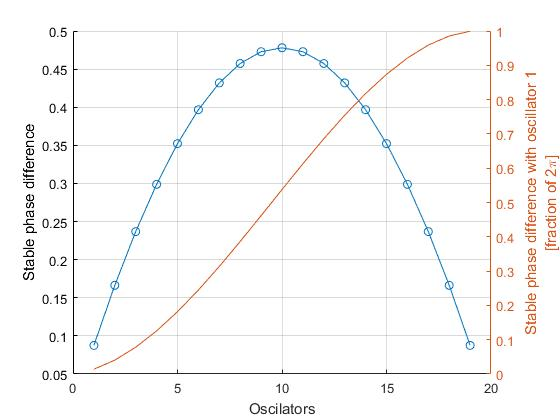
\includegraphics[width=\textwidth]{results/6.b/propaWavePhase.jpg}
		\caption{}
	\end{subfigure}
	\caption{Intrinsic and resulting frequencies for each oscillator (a). Stable phase difference between adjacent oscillator and with first oscillator (b). The simulation was performed with 20 oscillators, a coupling strength of 10 and a linear gradient of intrinsic frequencies with drift -0.092\,rad/step. These simulation parameters fulfill the phase locking condition.}\label{prop}
\end{figure}

\vspace{1cm}

\begin{figure}[!b]
	\centering
	\begin{subfigure}[b]{0.49\textwidth}
		\centering
		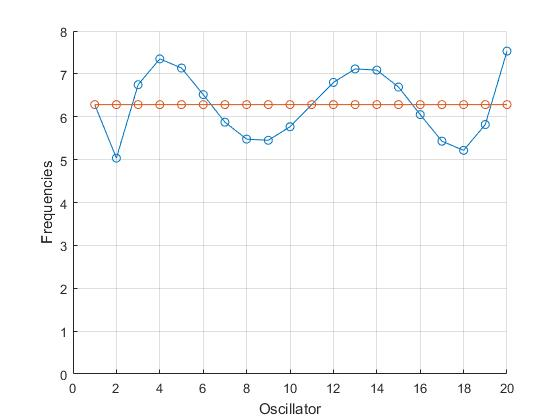
\includegraphics[width=\textwidth]{results/6.b/standWaveFreq.jpg}
		\caption{}
	\end{subfigure}
	\centering
	\begin{subfigure}[b]{0.49\textwidth}
		\centering
		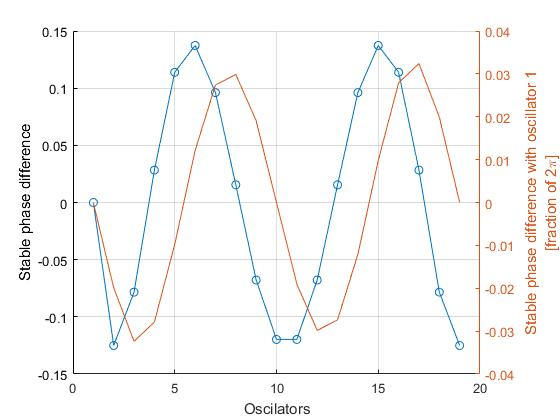
\includegraphics[width=\textwidth]{results/6.b/standWavePhase.jpg}
		\caption{}
	\end{subfigure}
	\caption{Intrinsic and resulting frequencies for each oscillator (a). Stable phase difference between adjacent oscillator and with first oscillator (b). The simulation was performed with 20 oscillators, a coupling strength of 10 and a polynomial gradient of intrinsic frequencies: $\omega_i = \omega_{1} + (-1.95\ 10^{-6}\times(i-1)^7 -1.37\ 10^{-4}\times(i-1)^6) -3.56\ 10^{-6}\times(i-1)^5 +4.12\ 10^{-2}\times(i-1)^4 -1.76\ 10^{-1}\times(i-1)^3 -2.43\ 10^{-1}\times(i-1)^2 +3.16\times(i-1)-4.02$. The simulation parameters fulfill the phase locking condition (i.e. the absolute value of the components of vector S are all inferior or equal to 1).}\label{stand}
\end{figure}

\begin{figure}[!b]
	\centering
	\begin{subfigure}[b]{0.49\textwidth}
		\centering
		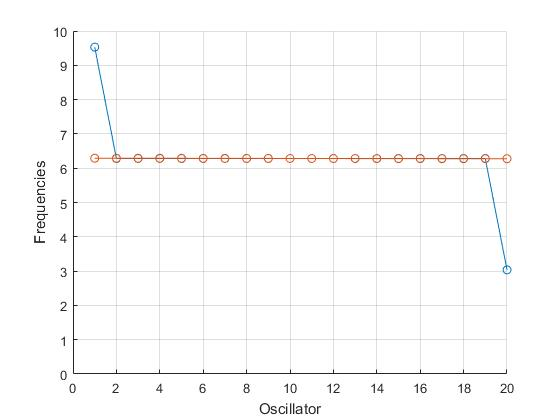
\includegraphics[width=\textwidth]{results/6.b/compSP_DP_CPFreq.jpg}
		\caption{}\label{3a}
	\end{subfigure}
	\centering
	\begin{subfigure}[b]{0.49\textwidth}
		\centering
		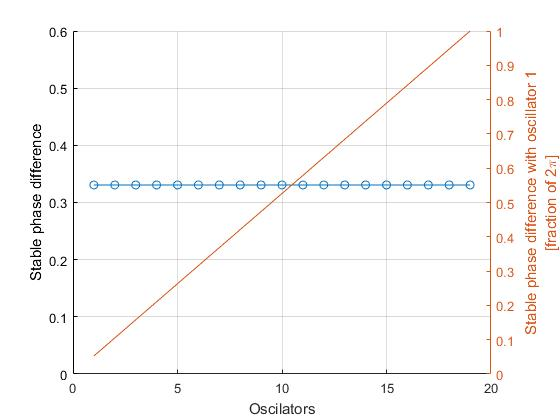
\includegraphics[width=\textwidth]{results/6.b/compSP_DP_CPPhase.jpg}
		\caption{}\label{3b}
	\end{subfigure}
	\centering
	\begin{subfigure}[b]{0.49\textwidth}
		\centering
		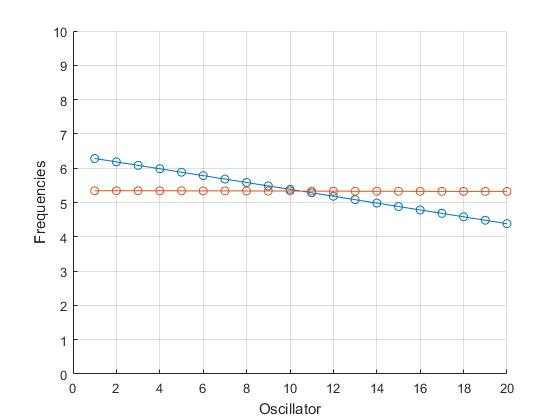
\includegraphics[width=\textwidth]{results/6.b/compSP_DP_DPFreq.jpg}
		\caption{}\label{3c}
	\end{subfigure}
	\centering
	\begin{subfigure}[b]{0.49\textwidth}
		\centering
		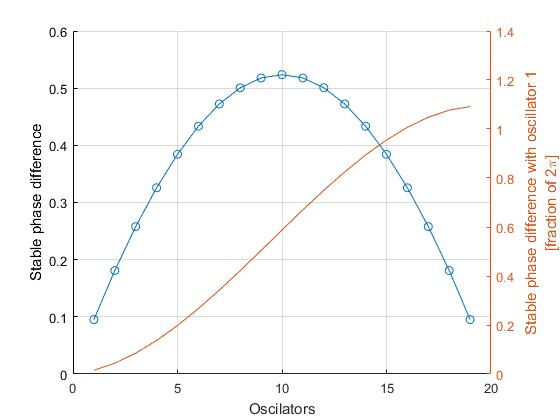
\includegraphics[width=\textwidth]{results/6.b/compSP_DP_DPPhase.jpg}
		\caption{}\label{3d}
	\end{subfigure}
	\begin{subfigure}[b]{\textwidth}
		\centering
		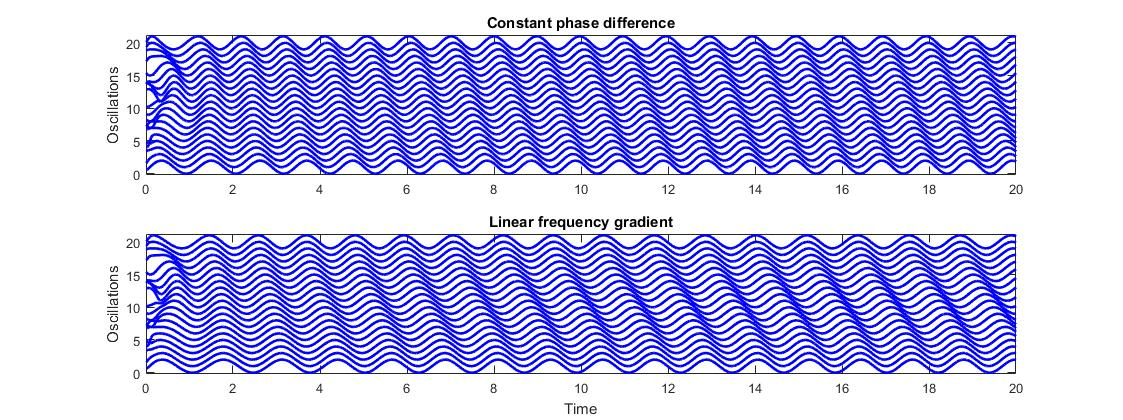
\includegraphics[width=\textwidth]{results/6.b/compSP_DP_oscillations.jpg}
		\caption{}\label{3e}
	\end{subfigure}
	\caption{Intrinsic and resulting frequencies for each oscillator (\ref{3a}, \ref{3c}). Stable phase difference between adjacent oscillator and with first oscillator (\ref{3b}, \ref{3d}). The simulations were performed for non linear gradient (\ref{3a}, \ref{3b}) given by: $\omega_{1} = 2\pi + 3.2469 ,\omega_{20} = 2\pi - 3.2469 , \omega_{i} = 2\pi$ for i = [2,19] and for a linear gradient (\ref{3c}, \ref{3d}) with drift -0.1\,rad/step. For all the simulations the number of oscillators was 20 and the coupling strength 10. The same initial conditions were used for both simulations. Simulated oscillation as a function of time (\ref{3e}) for both intrinsic frequency models.}
\end{figure}


\subsection{External load (6.c)}
In this part an external load with frequency $\omega_{mech}$ is applied to the tail of the lamprey with a sensory coupling strength $a_{sens}$:
\begin{align*}
\frac{d}{dt}\psi_N &= \omega_N + a \sin(\psi_{N-1}-\psi_N) + a_{sens} \sin(\omega_{mech}.t-\psi_N) \\
\frac{d}{dt}\mathbf{\phi} &= \mathbf{\Omega} + A \mathbf{S} - a_{sens} \sin(\omega_{mech}.t-\psi_N)\ [0, \ldots, 0,\, 1]'
\end{align*}
And therefore in phase locking regime:
\begin{align*}
\frac{d}{dt}\mathbf{\phi} &= 0\\
\mathbf{S} &= A^{-1}(a_{sens}\sin(\omega_{mech}.t-\psi_N)\ [0, \ldots, 0,\, 1]'-\mathbf{\Omega})
\end{align*}
The condition for phase locking is that for every element $s_i$ of $\mathbf{S}$: $|s_i|\leq1$.
Therefore setting the coupling strength to 10 and the frequency drift to -0.1\,rad/step, and as $-1\leq\sin(x)\leq1 \forall x \in \mathbf{R}$, we can calculate a value for the sensor coupling strength such that the condition for phase locking is verified.

We studied the effect of the sensor coupling strength and mechanical excitation frequency on the resulting frequency of the oscillators (see Figure \ref{4a} and \ref{4c}) while checking for phase locking conditions using the standard deviation of the phase differences between oscillators as a measure of phase locking (see Figure \ref{4b} and \ref{4d}). As expected, for the chosen set of parameters the standard deviation of the phase differences between the oscillators is bounded with small periodic perturbation corresponding to small variations of the few last oscillators. We can conclude that the system is in a phase locking regime in a less strict sense than in the previous sections.

From figure \ref{4c} one can observe that the effect of sensor coupling affects more strongly the last oscillator and that its resulting frequency converges towards the frequency of mechanical excitation. The frequency of the first oscillator also increases for high sensor coupling strengths.

From the figure \ref{4a} we can see that there is a range of excitation's frequencies ($0.8\times2\pi-0.95\times2\pi$\,rad/s) for which the last oscillator converges to $\omega_{mech}$ and the frequency of the first oscillator increases steadily. This range is close from the resulting frequency of the oscillator without mechanical excitation which is around $0.85\times2$. For higher excitations frequencies the frequency drops possibly because the intrinsic and excitation oscillations compensates each other. Neither the last nor the first oscillator frequencies converges toward $\omega_{mech}$ at higher mechanical excitation frequencies.
\newpage

\begin{figure}[h]
	\centering
	\begin{subfigure}[b]{0.49\textwidth}
		\centering
		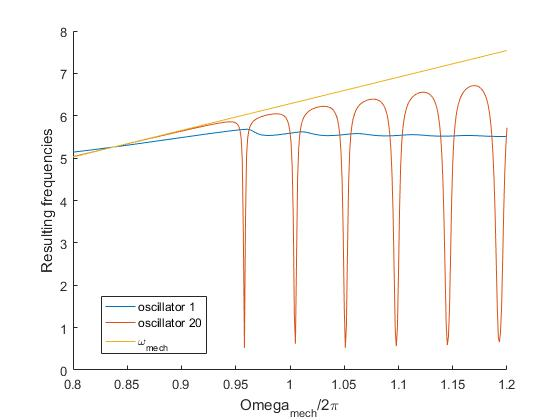
\includegraphics[width=\textwidth]{results/6.c/Freq_A_const.jpg}
		\caption{}\label{4a}
	\end{subfigure}
	\centering
	\begin{subfigure}[b]{0.49\textwidth}
		\centering
		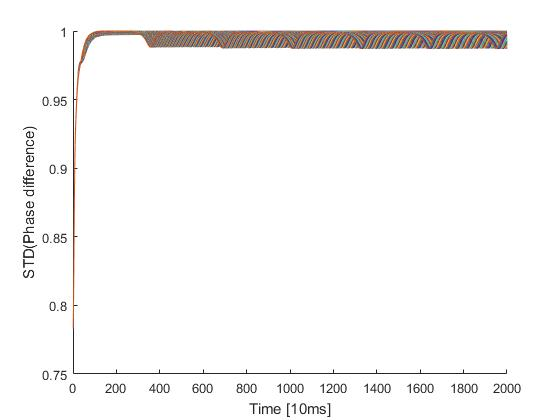
\includegraphics[width=\textwidth]{results/6.c/Phase_A_const.jpg}
		\caption{}\label{4b}
	\end{subfigure}
	\centering
	\begin{subfigure}[b]{0.49\textwidth}
		\centering
		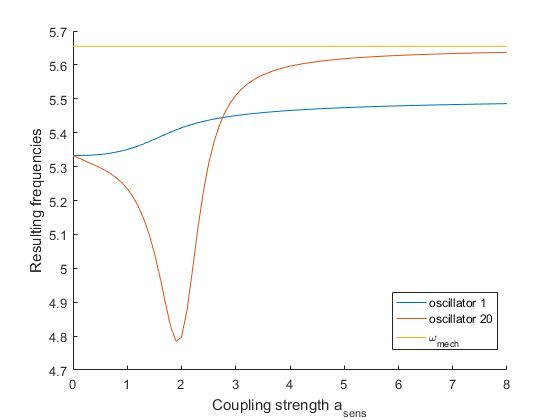
\includegraphics[width=\textwidth]{results/6.c/Freq_O_const.jpg}
		\caption{}\label{4c}
	\end{subfigure}
	\centering
	\begin{subfigure}[b]{0.49\textwidth}
		\centering
		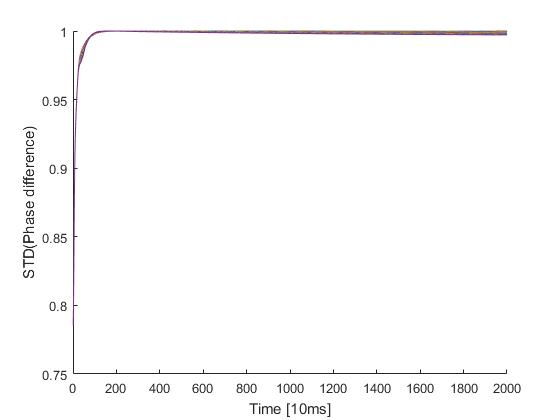
\includegraphics[width=\textwidth]{results/6.c/Phase_O_const.jpg}
		\caption{}\label{4d}
	\end{subfigure}
	\caption{Resulting frequencies of the oscillator 1 and 20 as well as mechanic excitation(\ref{4a}-\ref{4c}). In figure \ref{4a} the coupling strength was kept constant at 8 while the frequency of the mechanic excitation was varied. In figure \ref{4c} the mechanic excitation's frequency was kept constant while the coupling strength was varied. Figures \ref{4b} and \ref{4d} represent the normalized standard deviation of the phase difference between oscillators as a function of time to check for phase locking. All the simulations were done for models with coupling strength of 10, frequency drift of -0.1\,rad/step and 20 oscillators.}
\end{figure}

\FloatBarrier

\section{Comparing neuronal oscillators with phase oscillators}
\subsection{General behaviour (7.a)}

We saw  in the previous section that coupled phase oscillators could synchronize although they had different intrinsic frequencies and used this as a basis to model CPGs of the lamprey. Phase oscillators are a theoretical model however; it is thus of interest to find out, if the same results can be achieved using a more biological basis. This section was therefore devoted to study how coupled neuronal oscillators could produce the same type of CPGs as phase oscillators. A practical example could be 2 pendulums with an independant source of excitation coupled with a spring. If they have two intrinsic different frequency at the begining, there will be a transitory phase until they converge to the same freqency with some phase depending on the coupling strengh. The two signals in time look like sinusoidal curves. See figure \ref{2phase}.

\begin{figure}[!h]
	\centering
	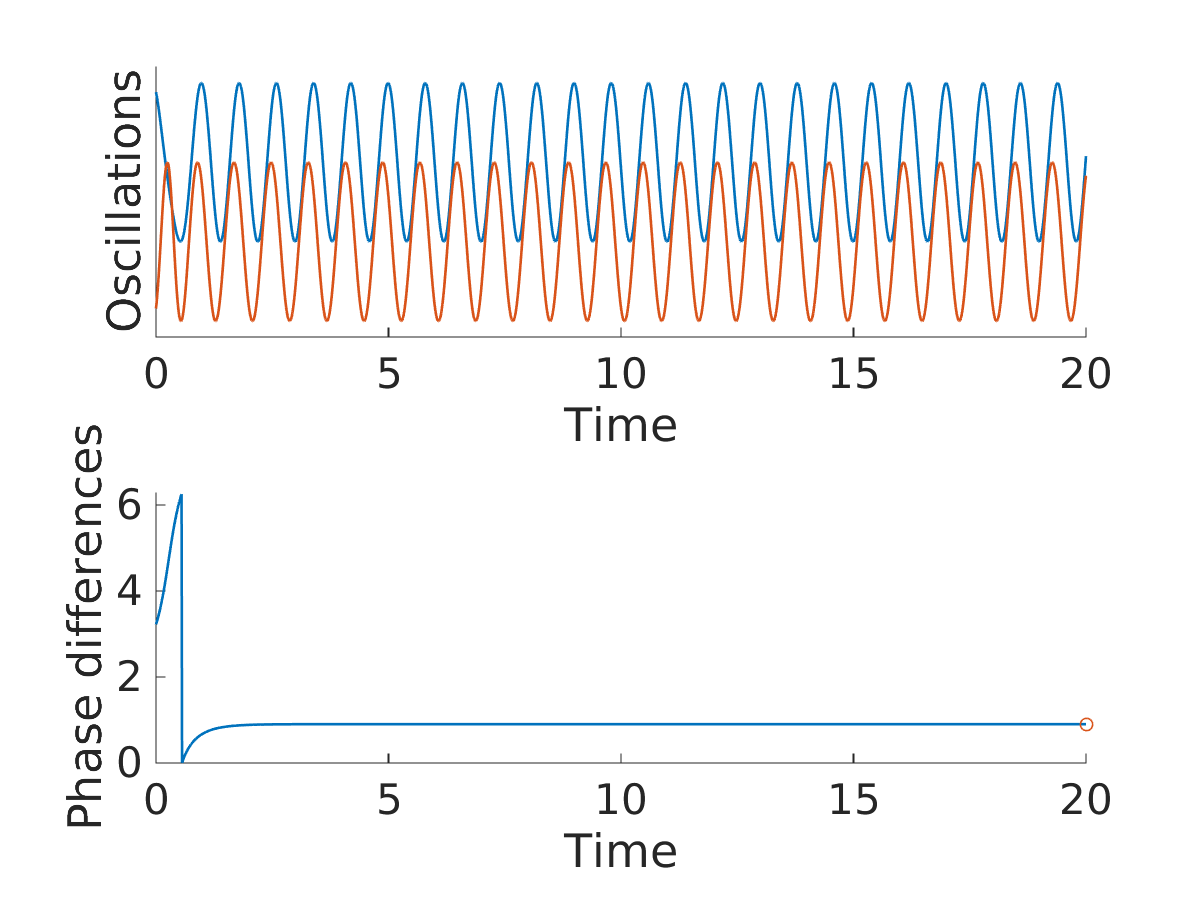
\includegraphics[width=0.5\textwidth]{fig/2phase.png}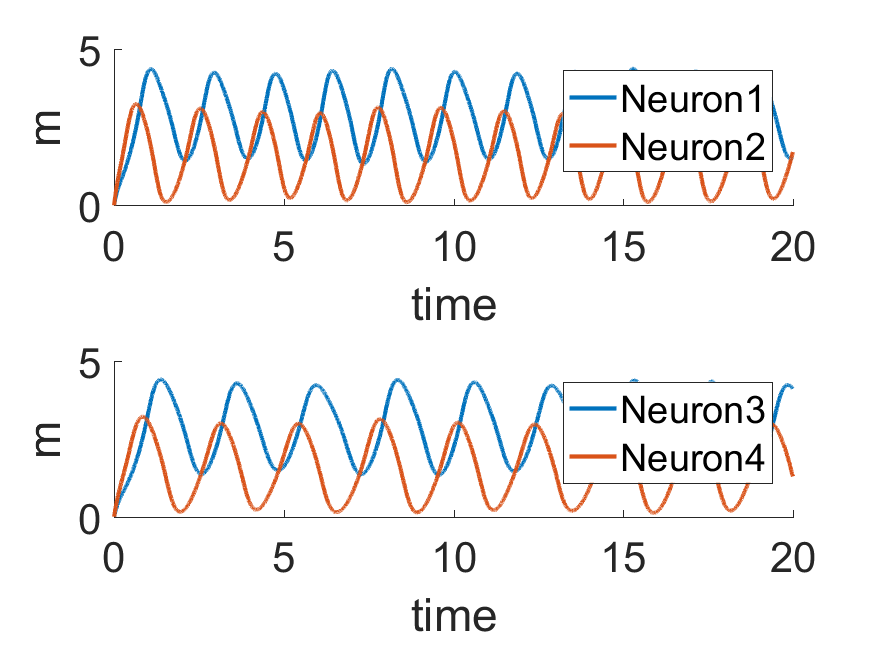
\includegraphics[width=0.5\textwidth]{fig/neuron1}
	\caption{On the left picture, a stable phase oscillator and some crazy stable neuronal oscillations using a strong negative coupling on the right picture.}\label{2phase}
\end{figure}

In opposition a phase oscillator, it is possible for a neuronal oscillator to reach different modes of stable oscillations even with some highly non linear curves using a high negative coupling strengh, see figure \ref{crazy}.

\begin{figure}[!h]
	\centering
	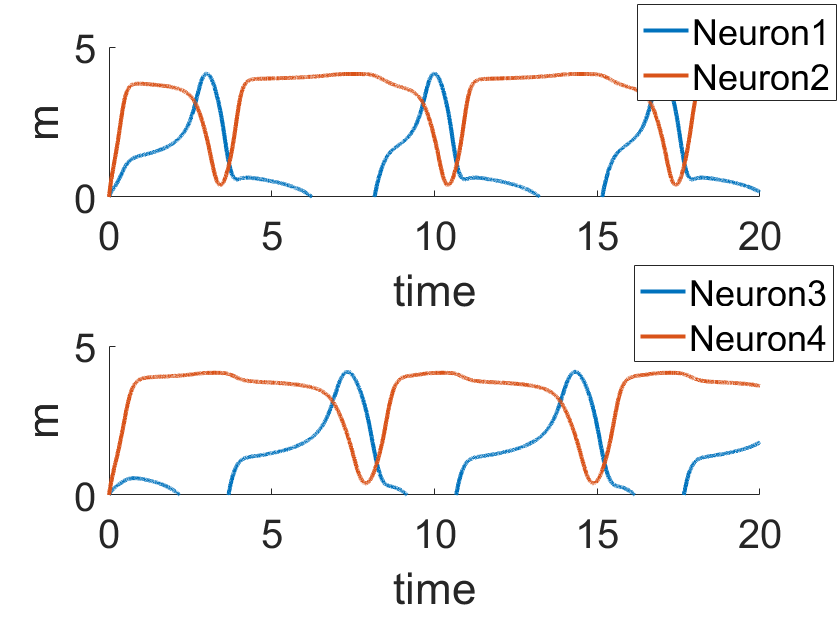
\includegraphics[width=0.5\textwidth]{fig/crazy.png}
	\caption{A stable neuronal oscillations using a strong negative coupling.}\label{crazy}
\end{figure}


When playing with the coupling strengh, one can observe two different behaviours. For the phase oscillators, a high coupling strengh results in the two masses oscillating at the same phase and frequency. If we add a strong positive coupling strengh to two neuronal oscillators, for example neuron 1 and 3, one can observe that the neurons will no longer oscillate but saturate to the maximum value because they excite one the other, see figure \ref{kill}. The neurons 2 and 4 will be killed because of the negative feedback from neurons 1 and 2.

\begin{figure}[!h]
	\centering
	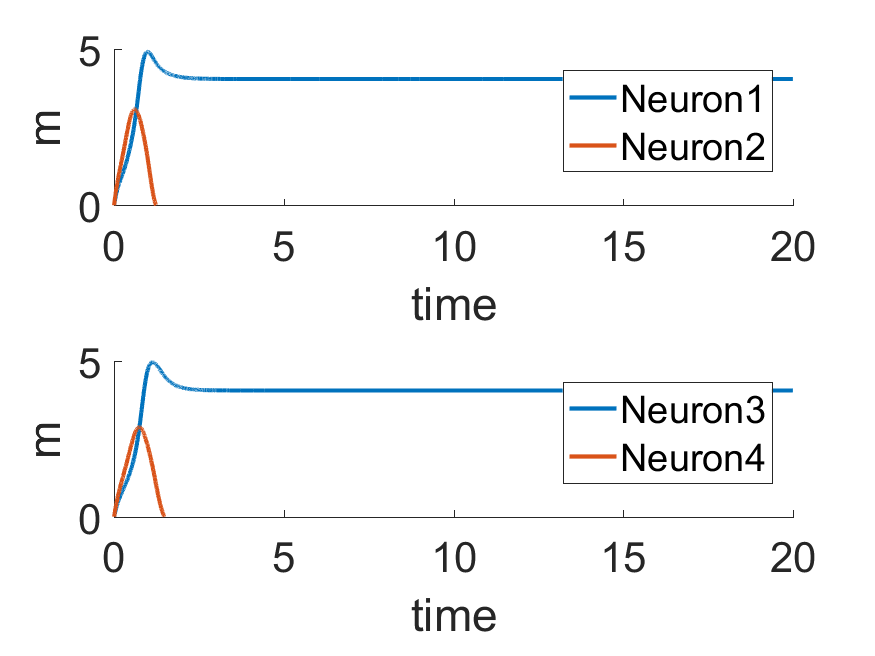
\includegraphics[width=0.5\textwidth]{fig/kill.png}
	\caption{Neurons with a high coupling strengh resulting in no oscillations.}\label{kill}
\end{figure}

\newpage

\subsection{Comparing forced oscillators (7.b)}

If the periodic input is in the same range of frequency as the neuron 1, one can distinguish two extrem cases. Firstly, if the coupling strengh is low, the neuron 3 will lightly feel the influence of the input periodic signal, see fig \ref{7b}.

\begin{figure}[!h]
	\centering
	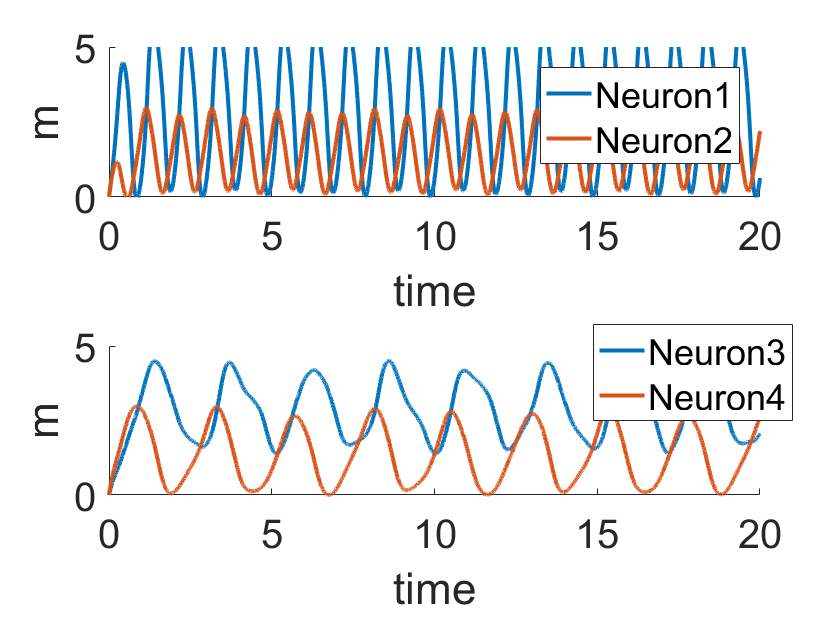
\includegraphics[width=0.5\textwidth]{fig/7b.png}
	\caption{Neuronal oscillators with a low coupling strengh and a periodic input on the first neuron.}\label{7b}
\end{figure}

Secondly, one can observe that even if the neurons are overconstrained and then saturate, there will be a residual oscillations, see fig \ref{sat}. This is interesting because we can imagine that the environement dictate the coupling strengh and our neuronal system could oscillate in different modes depending one the coupling strengh.

\begin{figure}[!h]
	\centering
	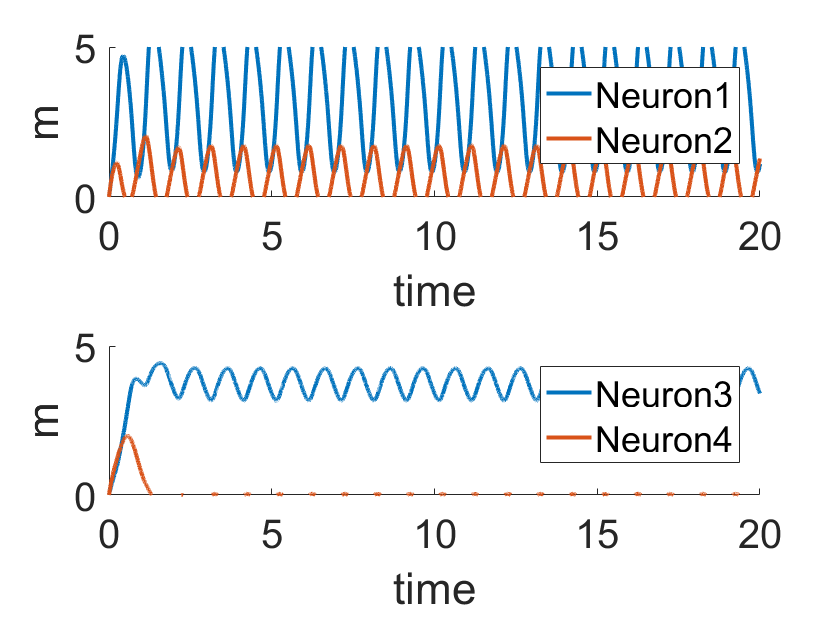
\includegraphics[width=0.5\textwidth]{fig/sat.png}
	\caption{A high positive coupling strengh on a neuronal oscillator excited by a periodic signal on the neuron 1.}\label{sat}
\end{figure}

\newpage

In the case where the frequency of the input signal is way higher than the instrinsic frequency, the transmition of the excitation for a both type of oscillators is low if the coupling strengh isn't too high. If the constrain is too high, the neuronal oscillator saturate as seen in the previous figure and the phase oscillator will have some chaotic behaviour. One can see on figure \ref{dd} that they have same kind of behaviour if one simulate the systems with parameters of the same order.

\begin{figure}[!h]
	\centering
	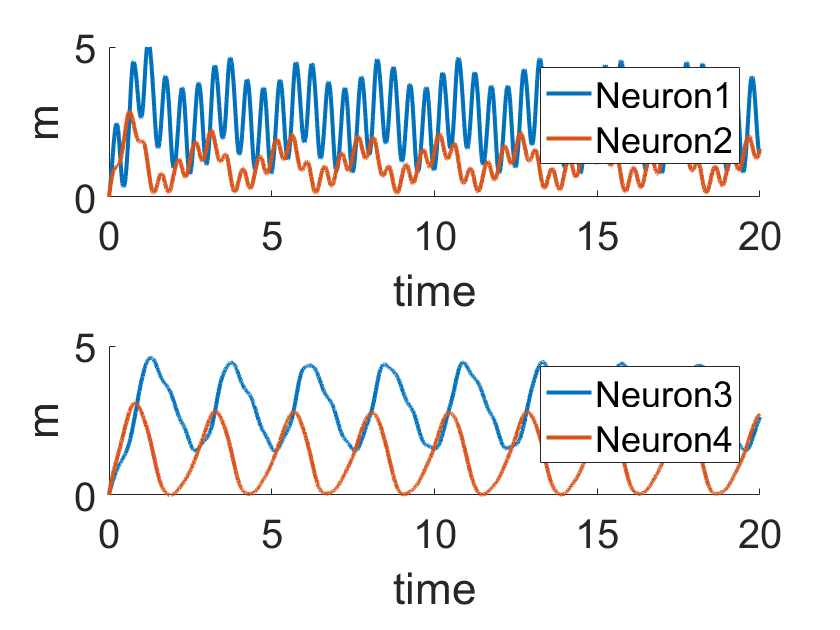
\includegraphics[width=0.5\textwidth]{fig/dd.png}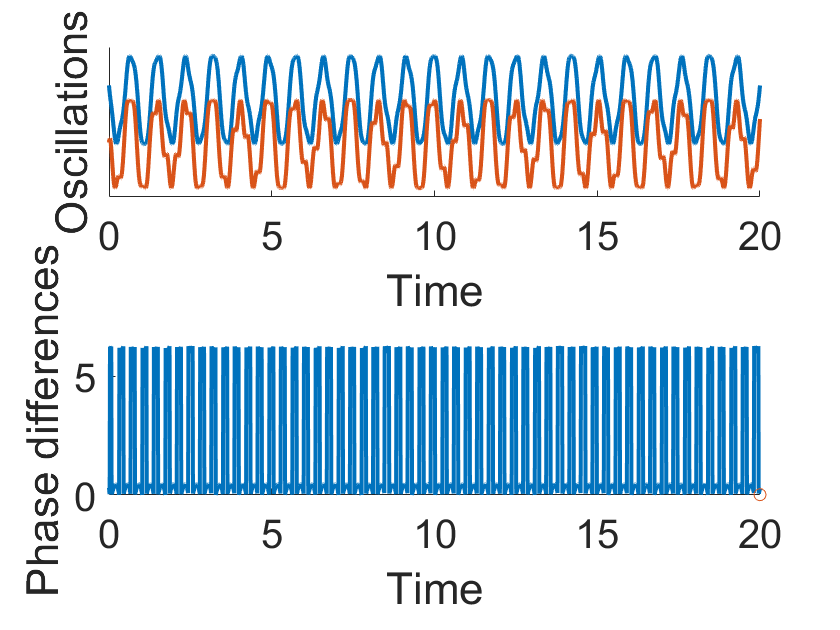
\includegraphics[width=0.5\textwidth]{fig/chao.png}
	\caption{On the left picture, a low constrain neuronal oscillator that doesnt saturate. On the right a chain phase oscillator with the same corresponding coupling strengh. In both case, a periodic input with a frequency 4 time higher than their intrinsic frequency is applied on one side.}\label{dd}
\end{figure}
	
\end{document}
